\documentclass{minimal}

\usepackage{tikz}
\usetikzlibrary{positioning}
\usetikzlibrary{intersections,decorations.pathreplacing,shapes,arrows}
\usetikzlibrary{plotmarks}
\usepackage{graphicx}
\begin{document}
\begin{tikzpicture}
  \node (A) {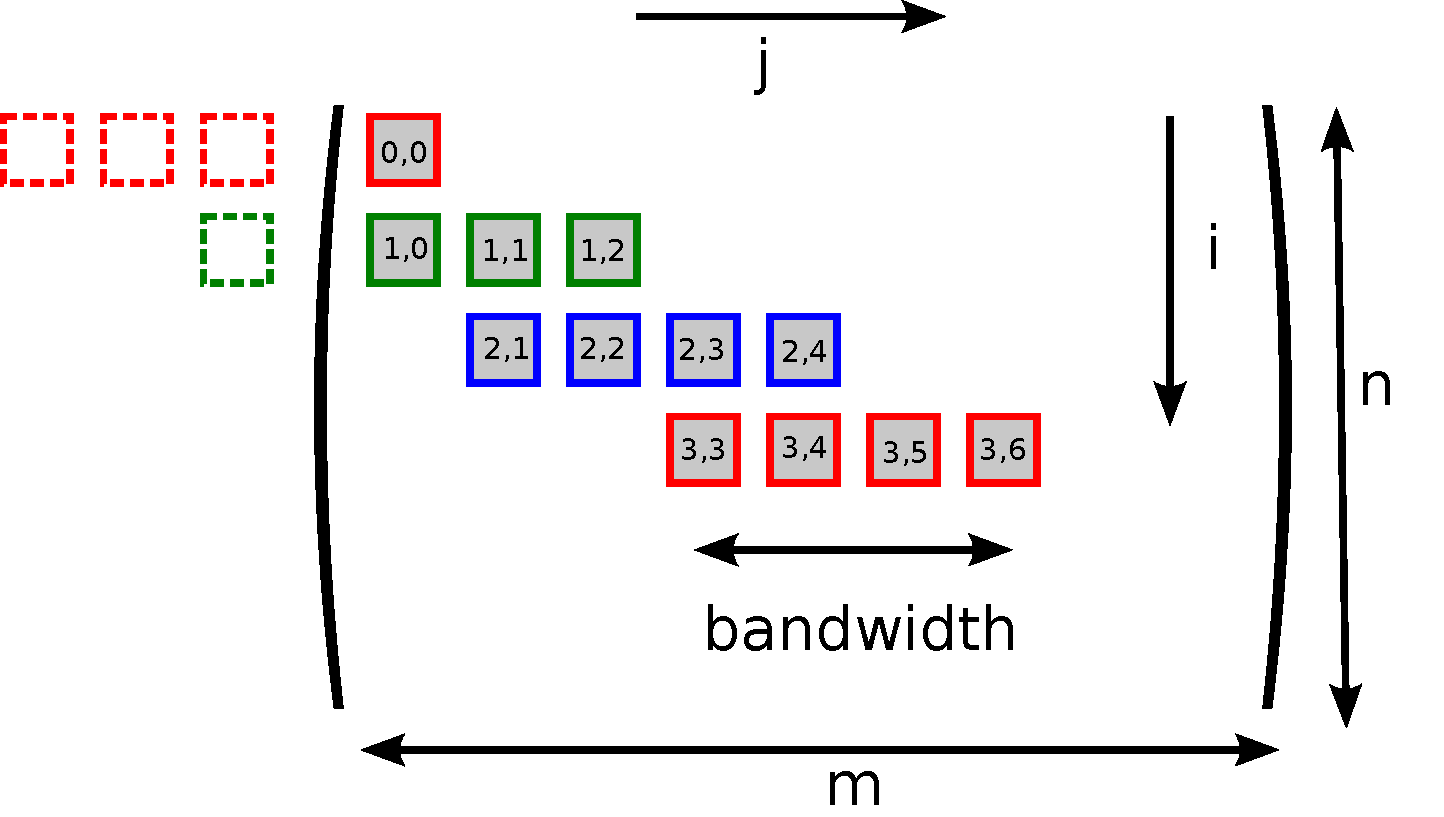
\includegraphics[height=5cm]{bandedmatrix}};
  \node (C) [right=of A.north east, anchor=north west] {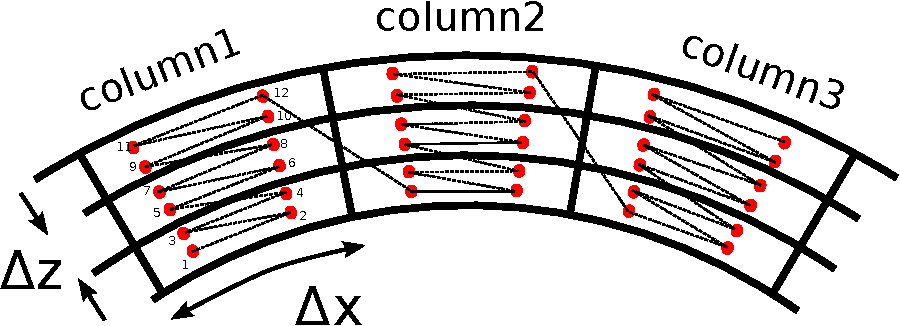
\includegraphics[width=7cm]{columndofs}};
  \node (B) [below=of C] {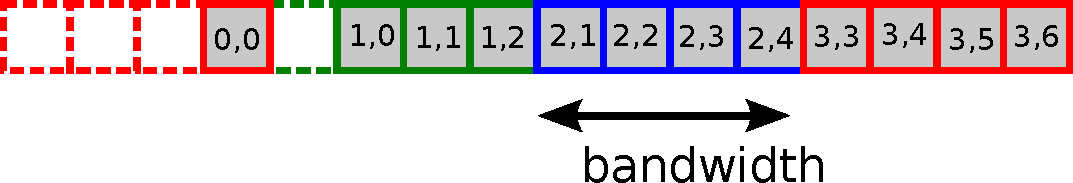
\includegraphics[height=1.2cm]{linearstorage}};
  \node (D) [above=of A.north east, anchor=south] {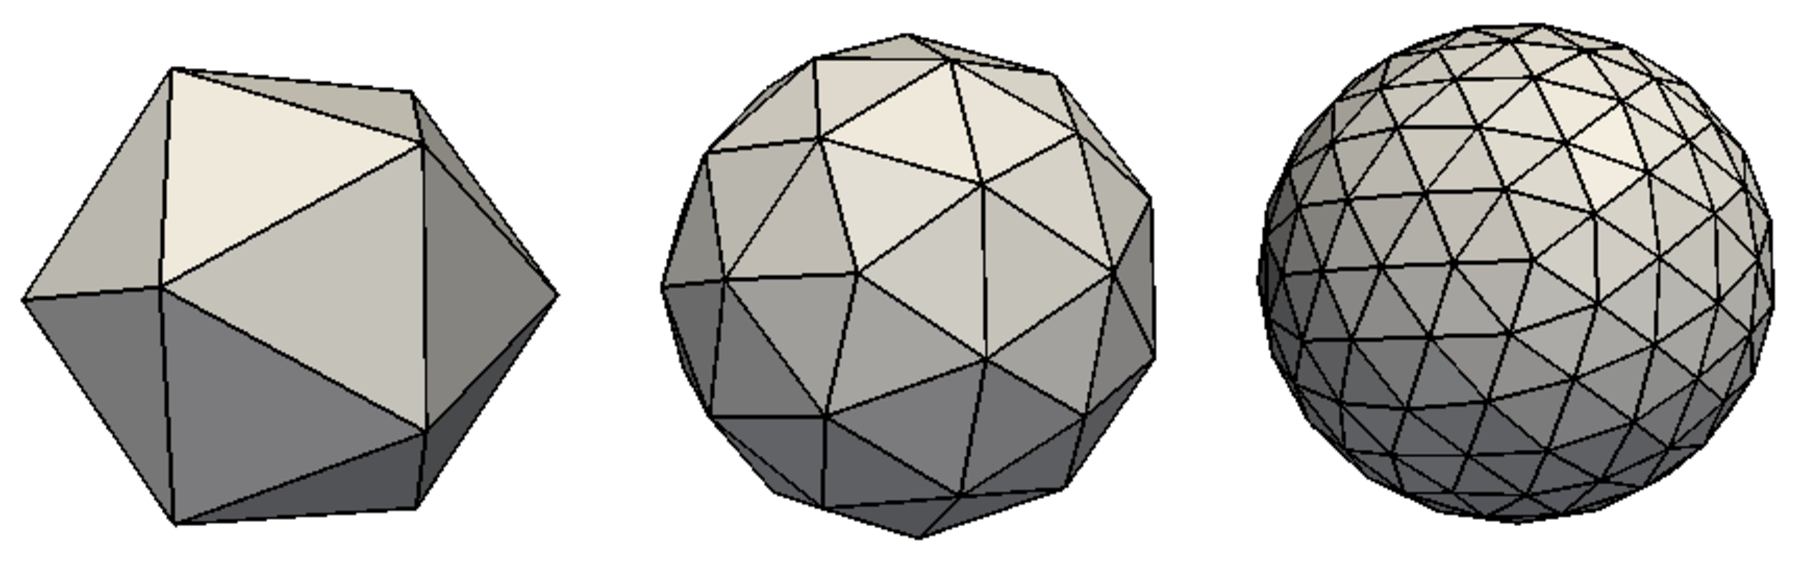
\includegraphics[width=7cm]{MeshHierarchy}};
\end{tikzpicture}
\end{document}
